\documentclass[12pt]{report}
\usepackage{amsmath}
\usepackage{amssymb}
\usepackage{keyval}
\usepackage{graphicx}
\newcommand{\Laplace}{\mathcal{L}}
\newcommand{\ft}{f(t)}
\newcommand{\ftn}[1]{f^{#1}(t)}
\newcommand{\FS}{F(S)}
\newcommand{\FSn}[1]{F^{#1}(S)}
\newcommand{\LaplaceIntegral}{\int_{0}^{-\infty}e^{-st}\ft\text{dt}}
\newcommand{\sbracket}[1]{\left[#1\right]}
\newcommand{\Y}{Y}
\newcommand{\Yn}[1]{y^{#1}(0)}
\newcommand{\fn}[1]{f^{#1}(0)}
\newcommand{\Sn}[1]{s^{#1}}
\newcommand{\LUx}[1]{\Laplace\sbracket{u_{#1}(x,t)}}
\newcommand{\Un}[2]{u_{#1}(#2)}
\newcommand{\LInt}{\int_{0}^{\infty}e^{-st}u(x,t)\text{dt}}
\newcommand{\LFt}{\Laplace \sbracket{\ftn{}}}
\newcommand{\NI}{\noindent}
\newcommand{\LFn}[1]{\Laplace \sbracket{#1}}
\newcommand{\Dtl}[1]{\Delta_{#1}}
\newcommand{\sqL}[1]{#1^{2}}
\newcommand{\sqLn}[2]{#1^{#2}}
\newcommand{\psq}{\pi^{2}}
\newcommand{\psqn}[1]{\pi^{#1}}
\newcommand{\InverseL}[1]{\Laplace^{-1}\left[#1\right]}
\newcommand{\LT}[1]{\Laplace \left[#1\right]}
\newcommand{\LTb}[1]{\Laplace \left(#1\right)}
\newcommand{\Unx}[1]{\Un{#1}{x,t}}
\newcommand{\InverseLx}[1]{\Laplace^{-1}\left\{ #1 \right\}}
\newcommand{\Usub}[1]{u_{#1}}
\newcommand{\Usup}[1]{u^{#1}}
\newcommand{\bt}[1]{\textbf{#1}}
\newcommand{\refn}[1]{\bt{(\ref{#1})}}

\renewcommand{\baselinestretch}{1.5}
\begin{document}
\pagenumbering{roman}
\begin{titlepage}
\addcontentsline{toc}{section}{\numberline{}Title Page}
\begin{center}
{\bf APPLICATION OF LAPLACE TRANSFORM AND MODIFIED VARIATIONAL ITERATION METHOD IN SOLVING SECOND ORDER PARTIAL DIFFERENTIAL EQUATIONS }
\end{center}
$$$$
\begin{center}
    \textbf{\itshape\large BY}
    \end{center} 
$$$$
\begin{center}
	{\bf FRANCIS, Omoniyi Emmanuel\\
							17/56EB104}
	\end{center}
$$$$
\begin{center}
   \textbf{A PROJECT SUBMITTED TO THE
    DEPARTMENT OF MATHEMATICS, FACULTY OF PHYSICAL SCIENCES,
    UNIVERSITY OF ILORIN, ILORIN, NIGERIA,
    $$$$
     IN PARTIAL 
    FULFILMENT OF REQUIREMENTS FOR THE AWARD OF
    BACHELOR OF SCIENCE {\itshape{(B.Sc.)}} DEGREE IN MATHEMATICS.}
\end{center}
$$ $$ 
\\ \\
\begin{center}
	{\bf 	JUNE 2021}
\end{center}
\end{titlepage}
\newpage

		\section*{\begin{center}	\textbf{\Large Certification}   \end{center}}
		\addcontentsline{toc}{section}{\numberline{}Certification}
 This is to certify that this project was carried out by \textbf{FRANCIS, Omoniyi Emmanuel} of Matriculation Number  \textbf{17/56EB104}, for the award of Bachelor of science B.Sc (Hons) degree in the Department of Mathematics, Faculty of Physical sciences, University of Ilorin, Ilorin, Nigeria.
\\
\\
................................... \qquad \qquad\qquad\qquad\qquad...................... \\
PROF. IDOWU A.S   \qquad\qquad\qquad\qquad\qquad\qquad Date\\
(SUPERVISOR)\\
\\
\\
\\
...................................... \qquad\qquad\qquad\qquad\quad ......................\\
PROF. K. RAUF      \qquad\qquad\qquad\qquad\qquad\qquad\qquad     Date\\
(HEAD OF DEPARTMENT)\\
\\
\\
\\
..................................... \qquad\qquad\qquad\qquad\qquad .......................\\
EXTERNAL EXAMINER \qquad\qquad\qquad\qquad\qquad\quad         Date\\

\newpage
		\section*{\begin{center}	\textbf{\Large Dedication}   \end{center}}
		\addcontentsline{toc}{section}{\numberline{}Dedication}
First and foremost, this project work is dedicated to Almighty God who has brougth me this far in my B. Sc. program, and also to my dearest parents Mr. and Mrs. Francis, and Mr. and Mrs. Oladapo, and as well to my siblings. I cannot but also dedicate this work to all the Mathematics lecturers who has in one way or the other impacted into me.
\newpage						\section*{\begin{center}	\textbf{\Large Acknowledgments}   \end{center}}
						\addcontentsline{toc}{section}{\numberline{}Acknowledgments} 					

All glory and honour belong to Almighty God for His loving kindness and mercy which He bestowed on me, His presence in the course of my journey and for the ability He has given me to write this project.\\

\par Furthermore, with humility and respect I appreciate the effort of my hardworking supervisor, Prof. A.S. Idowu for his unlimited guidance and fatherly advice while carrying out this project work. 

\par I also appreciate my amiable and relentless Head of Department Prof.
K. Rauf and my amiable Level Adviser (LA), Dr. (Mrs.) I.F. Usamot for their words of encouragement, concern and support. \\

Also, I appreciate all my amazing lecturers who have taught me well enough namely; Prof. J.A. Gbadeyan, Prof. T.O. Opoola, Prof. O.M. Bamigbola, Prof. M.O. Ibrahim, Prof. O.A. Taiwo, Prof. R.B. Adeniyi, Prof. K.O. Babalola, Prof. M.S. Dada, Doctors; E.O. Titiloye, O.A. Fadipe-Joseph, Y.O. Aderinto, C.N. Ejieji, B.M. Yisa, J.U. Abubakar, K.A. Bello, G.N. Bakare, B.M. Ahmed, O.T. Olootu, D.A. Uwaheren, O. Odetunde, T.L. Oyekunle, A.A. Yeketi.\\

The efforts of the non-academic staff of the department of mathematics are equally appreciated.\\

May God in His infinite mercy reward you all and your families for your
contribution towards my academic success.
\par Finally, I say a very big shout out to my colleagues and friends in the department, may Almighty  God increase His blessings and mercies towards you all (Amen).

 \newpage
	\section*{\begin{center}	\textbf{\Large Abstract}   \end{center}}
						\addcontentsline{toc}{section}{\numberline{}Abstract}
\upshape 
In this project, the solution of Partial Differential Equations using Laplace Transform is presented. In addition to the laplace transform method, the new modified variational iteration method was introduced. A safe combination of Laplace Transform and the new modified variation iteration method was considered to solve both the linear and nonlinear aspect of Partial Differential Equations.
\addcontentsline{toc}{section}{\numberline{}Table of Contents}
\tableofcontents
    \newpage
 \pagenumbering{arabic}
\chapter{HISTORICAL BACKGROUND OF DIFFERENTIAL EQUATIONS}
\section{INTRODUCTION}
\qquad In mathematics, history of differential equations traces the development of “differential equations'' from calculus, itself independently invented by English physicist Isaac Newton and German mathematician Gottfried Leibniz. The history of the subject of differential equations, in concise form, from a synopsis of the recent article “The History of Differential Equations, 1670-1950 (Archibald et al., 2005). 
\par Differential equations began with Leibniz, the Bernoulli brothers(Jacob \& Johann Bernoulli), not long after Newton’s ‘fluxional equations’ in the 1670s. Differential equations differ from ordinary equations of mathematics in that in addition to variables and constants they also contain derivatives of one or more of the variables involved (Archibald et al., 2005).

\par In circa 1671, English physicist Isaac Newton wrote his then-unpublished. “The Method of Fluxions and Infinite Series”(published in 1736), in which he classified first order differential equations, known to him as fluxional equations, into three classes, as follows (using modern notation):
\par Ordinary differential equations
\begin{align*}
&\frac{dy}{dx}=f(y)\tag{Class 1}
\end{align*}
\begin{align*}
&\frac{dy}{dx}=f(x,y)\tag{Class 2}
\end{align*}
\par Partial differential equations
\begin{align*}
& x \frac{\partial u}{\partial x}+ y\frac{\partial u}{\partial y}=u\tag{Class 3}
\end{align*}
The first two classes contain only ordinary derivatives of one or more dependent variables, with respect to a single independent variable, and are known today as “ordinary differential equations”; the third class involves the partial derivatives of one dependent variable and today are called ``partial differential equations'' (Blurnan, 1989).

\par The study of “differential equations”, according to British mathematician Edward Ince, is said to have began in 1675, when German mathematician Gottfried Leibniz wrote the following equation (date of introduction of integral sign; see: symbols):
\newpage
\begin{align*}
\int x dx = \frac {1}{2}x^2
\end{align*}
\par In 1676, Newton solved his first differential equation. That same year, Leibniz introduced the term “differential equations” (aequatio differentialis, Latin) or to denote a relationship between the differentials dx and dy of two variables x and y (Alfred, 1994).

In 1693, Leibniz solved his first differential equation and that same year Newton published the results of previous differential equation solution methods—a year that is said to mark the inception for the differential equations as a distinct field in mathematics (Alfred, 1994).

The Italian mathematician's book in 1707 titled “On the Construction of First-degree Differential Equations”, written between 1701 and 1704, was the firt book on the subject of differential equation published in Latin. The book was largely based or themed on the views of the Leibniz and the Bernoulli brothers. Most of the publications on differential equations and partial differential equations, in the years to follow, in the 18th century, seemed to expand on the version developed by Leibniz, a methodology, employed by those as Leonhard Euler, Daniel Bernoulli, Joseph Lagrange, and Pierre Laplace.  Swiss mathematician Leonhard Euler ,(1739) began using the integrating factor as an aid to derive differential equations that were integrable in finite form (Denis, 2020).\\

Denis (2020) revealed that the Euler-Lagrange equation was developed in the 1750s by Euler and Lagrange in connection with their studies of the tautochrone problem. This is the problems of determining a curve on which a weighted particle will fall to a fixed point in in a fixed amount of time, independent of the starting point. Lagrange solved this problem in 1755 and sent the solution to Euler. Both further developed Lagrange's method and applied it to mechanics, which led to the formulation of Lagrangian mechanics.\\

In 1822, Fourier published his work on heat flow in Theorie analytique de la chaleur (The Analytic Theory of Heat), in which he based his reasoning on Newton's law of cooling, namely, that the flow of heat between two adjacent molecules is proportional to the extremely small difference of their temperatures. Contained in this book was Fourier's proposal of his heat equation for conductive diffusion of heat. This partial differential equation is now taught to every student of mathematical physics (Denis, 2020).

\subsection {Types of differential equations}
There are two types of differential equations
\begin{enumerate}
	\item[i.] \textbf{Ordinary Differential Equation:} A differential equation involving derivatives with respect to a single independent variable is called an ordinary differential equation (Sikka, 2018).
  \item[ii.] \textbf{Partial Differential Equation:} A differential equation involving partial derivatives with respect to more than one independent variables. 
\end{enumerate}
\subsection{Order of Differential Equation}
\qquad The highest order derivative present in the differential equation (ordinary differential equation and partial differential equation) is the order of the differential equation (Sikka, 2018).
\\
For example
\begin{align*}
& \frac{\partial u}{\partial x}=u+xy \tag{i}\\
& \left (\frac{\partial u}{\partial x}\right)+ \frac{\partial^3u}{\partial y^3}=2x\left(\frac{\partial u}{\partial x}\right) \tag{ii} \\
& \frac{\partial^2u}{\partial x^2}=\left(1+\frac{\partial u}{\partial x}\right)^{\frac{1}{2}}\tag{iii}
\end{align*}
The first equation is of order one (first order), the second is of order three (third order) while the third equation is of order two (second order).
\subsection{Degree of Differential Equation}
\qquad The degree of a differential equation is the highest power of  the highest order derivative which occurs in the differential equation after the equation has been rationalized i.e. made free of radicals and fractions (Sikka, 2018).\\
For example
\begin{align*}
& \frac{\partial u}{\partial x}=u+xy\tag{i}\\
& \frac{\partial u}{\partial x}+ \frac{\partial u}{\partial y}+\frac{\partial u}{\partial z}=xyz\tag{ii}\\
& \frac{\partial^2u}{\partial x^2}=\left(1+\frac{\partial u}{\partial x}\right)^{\frac{1}{2}}\tag{iii}
\end{align*}
Equation (i) and (ii) are of first degree while equation (iii) is of second degree
\section{Partial differential equations (PDE)}
Partial differential equations are those equations which contain partial differential coefficients, independent and dependent variables. The independent variables will be denoted by $x \mbox{ and } y \mbox{ and the dependent variable by } z$ (Solin, 2005).\\
\subsection {Classification of partial differential equation}
\par The second order linear partial differential equations can be classified into three (3); namely:
\begin{enumerate}
	\item[i.] Elliptic PDE 
	\item[ii.] Parabolic PDE 
	\item[iii.] Hyperbolic PDE 
\end{enumerate}

\par Consider the second order linear PDE in two variables
\begin{equation}
Au_{xx} + Bu_{xy} +Cu_{yy} +Du_x+ Eu_y+ Fu=G
\end{equation}
The discriminant\\
\begin{equation*}
\quad d=B^2(x_0,y_0) - 4A(x_0,y_0)C(x_0,y_0)\\
\end{equation*}
At $(x_0, y_0)$,the equation is said to be \\

\begin{enumerate}
	\item[i.] Elliptic if $d<0$
	\item[ii.] Parabolic if $d=0$
	\item[iii.] Hyperbolic if $d>0$
\end{enumerate}

If this is true at all points in a domain, then the equation is said to be elliptic, parabolic, or hyperbolic
in that domain.\\
If there are n independent variables $x_1, x_2, ..x_n$, a general linear partial differential equation of second order has the form.\\
\begin{equation*}
\sum \sum a_{i,j}u_{xixj} \quad \text{plus lower order terms} = 0 \\
\end{equation*}
The classification depends upon the signature of the eigenvalues of the coefficient matrix; see below: \\
\begin{enumerate*}
	\item i. Elliptic: The eigenvalues are all positive or all
	negative.
	\item ii. Parabolic : The eigenvalues are all positive or all negative, save one which is zero.
	\item iii. Hyperbolic: There is only one negative eigenvalue and all the rest are positive, or
	there is only one positive eigenvalue and all the rest are negative (Solin, 2005).
\end{enumerate*}

\subsection {Examples of partial differential equation}
Examples of partial differential equations include:
\begin{align*}
& \frac{\partial u}{\partial x}=2u \\
& x \frac{\partial^2u}{\partial x^2}-\frac{\partial^2u}{\partial y^2}=0
\end{align*}
The partial differential coefficients are denoted as follows
\begin{align*}
 \frac{\partial z}{\partial x}=p, \frac{\partial z}{\partial y}=q, \frac{\partial^2z}{\partial x^2}=r,
\frac{\partial^2z}{\partial x \partial y}=s, \frac{\partial^2z}{\partial y^2}=t
\end{align*}
\section{Aim And Objectives Of The Project}
\qquad The aim of this project is to effectively solve partial differential equations (linear and non-linear) using the Laplace Transform method and the modified He's variational iteration method. The objectives are to:
\begin{enumerate}
	\item[i.] solve partial differential equations;
  \item[ii.] explain linear and non-linear partial differential equations;
  \item[iii.] use Laplace transform method and the new modified variational method to solve partial differential equation (linear and non-linear, 2nd order);
	\item[iv.] to perform a comparative study on the introduced method  in (iii) above and a numerical solution of partial differential equation; and
	\item[v.] and to show where and why to use the laplace transform with the new modified variational method.
\end{enumerate}
\chapter{LITERATURE REVIEW}
\qquad The study of partial differential equation (PDEs) started in the 18th century in the works of Euler, D'Alembert, Lagrange and Laplace as a central tool in the description of mechanics of series of  things that are slightly different from each other and more generally, as the principal mode of analytical study of models in the physical science. The analysis of physical models has remained to the present day as one of the fundamental concerns of the development PDEs. Beginning in the middle of the 19th century, particularly with the work of Riemann, PDEs also became an essential tool in other branches of mathematics (Poincare, 1890).\\
\par Poincare (1890) gave the first complete proof in rather general domain of the existence and uniqueness of a solution of the Laplace equation for any Dirichlet boundary condition. He introduced the so called Balayage method, this iteration method relies on solving the Dirichlet problem on balls in the domain and makes extensive use of the maximum principle and Harnack's inequality for harmonic functions.\\
\par Some important Partial Differential Equations in sciences and Engineering:
\begin{enumerate}
	\item[i.] Wave Equation
  \begin{equation}
  \frac{\partial ^2 u}{\partial t^2}-c \frac{\partial^2u}{\partial x^2}=0
  \end{equation}
  \item[ii.] Laplace Equation
  \begin{equation}
  \frac{\partial^2 u}{\partial x^2}+\frac{\partial^2 u}{\partial y^2}=0
  \end{equation}
  \item[iii.] Poisson's Equation
  \begin{equation}
  \frac{\partial^2 u}{\partial x^2}+\frac{\partial^2 u}{\partial y^2}=f(x,y), \mbox{ where } f(x,y) \mbox{ is a given function}
  \end{equation}
  \item[iv.] Helmholtz Equation
  \begin{equation}
  \frac{\partial^2 u}{\partial x^2}+\frac{\partial^2 u}{\partial y^2}+ku^2=0
  \end{equation}
  \end{enumerate}
\subsubsection{Essential concepts of Differential Equation}
\qquad All problems in science and engineering have their own specific mathematical approaches. A differential equation can be solved using many approaches in which Laplace transform is one of them. \\
\newpage
\par The Laplace transform is named after a french mathematician, astronomer and statistician Pierre-Simon Laplace, who used a similar transform (now called z transform) in his work on probability theory. The current widespread use of the transform came about soon after world war II, although it has been used in 19th century by Abel, Lerch, Heaveside and Bromwich. From 1744, Leonard Euler investigated integrals of the form:
\begin{equation}
z=\int X(x)e^{at}~dx \mbox{ and } z=\int X(x)x^A~dx
\end{equation}
as solutions of differential equations but did not pursue the matter very far (Williams, 1973).\\

Furthermore, Laplace transform is a mathematical operation that is used to transform a variable (such as $x \mbox{ or } y \mbox{ or } t$) to a parameter(s). \\
mathematically, it can be expressed as
\begin{equation}
L[f(t)]=\int_0^\infty e^{-st} f(t)dt=F(s)
\end{equation}
where $F(s)=$ expression of Laplace transform of function $f(t)$. \\
Williams (1973) revealed that the Laplace transform is used to transform a variable in a function into a parameter. So, after the transformation, that variable is no longer available anymore, but should be treated as a parameter.
\chapter{LAPLACE TRANSFORM AND VARIATION ITERATION METHOD}
\section{LAPLACE TRANSFORM AND ITS PROPERTIES}
\par Laplace transformation helps in solving the differential equations with boundary values without finding the general solution and the value of the arbitrary constants.
\subsection{METHOD OF LAPLACE TRANSFORM}
\textbf{Definition}: Let $f(t)$ be function defined for all positive values of $t$, then

\begin{equation}
F(s)= \int^\infty_0 e^{-st}f(t)dt
\end{equation}
provided the integral exists, is called the laplace transform of $f(t)$. It is denoted as
\begin{equation}
L[f(t)]=F(s)= \int^\infty_0 e^{-st}f(t)dt
\end{equation}

\textbf{Laplace transform of some elementary functions}
\subsubsection{Example 1:} Find the Laplace transform of $f(t)=c, 0 \leq t \leq \infty$ i.e. $L[c]$, where $c$ is a constant.
\\ \textbf{solution} \\
Let,
\begin{eqnarray}
L[f(t)]&=&\int^\infty_0 e^{-st}f(t)dt \\
L[C]&=&\int^\infty_0 e^{-st}C dt \nonumber \\
&=& C\int^\infty_0 e^{-st}dt \nonumber\\
&=& C \left[\frac{e^{-st}}{-s} \right]_0^\infty \nonumber\\
&=& -\frac{C}{s} \left[e^{-st}\right]_0^\infty = -\frac{C}{s}\left[0-1\right]= \frac{c}{s}
\end{eqnarray}
If $c=1, l[1]= \frac{1}{s}, c=2, L[2] = \frac{2}{s}, c=3, L[3]=\frac{3}{s}$
\subsubsection{Example 2}
Find the Laplace transform of $f(t)=t^n, 0 \leq t \leq \infty $ where $n \mbox{ and } s$ are positive
\subsubsection{solution} 
\begin{equation}
L(t^n)= \int_0^\infty e^{-st}t^n dt
\end{equation}
putting $st=x \Rightarrow t=\frac{x}{s} \Rightarrow dt= \frac{dx}{s}$. \\
Thus, we have
\begin{eqnarray}
L(t^n)&=& \int_0^\infty e^{-x}\left(\frac{x}{s}\right)^n \frac{dx}{s} \nonumber\\
&=&\frac{1}{s^{n+1}} \int_0^\infty e^{-x}x^ndx \nonumber\\
&=& \frac{n!}{s^{n+1}}
\end{eqnarray}
\textbf{Note}
\begin{eqnarray}
\Gamma(n+1) &=& \int_0^\infty e^{-x}.x^n dx ~~~~~~~~~~\mbox{ and } \nonumber\\
\Gamma(n+1) &=& n!
\end{eqnarray}

\subsubsection{Example 3}
Find the Laplace transform of $f(t)=e^{at} \mbox{ where } s> a$
\subsubsection{solution}
\begin{eqnarray}
L[e^{at}]&=& \int_0^\infty e^{-st}.e^{at}dt = \int_0^\infty e^{-st+at}dt\nonumber \\
&=& \int_0^\infty e^{(-s+a)t}dt = \int_0^\infty e^{-(s-a)t}dt\nonumber \\
&=& \left[\frac{e^{-(s-a)t}}{-(s-a)}\right]_o^\infty = -\frac{1}{s-a}\left[\frac{1}{e^{(s-a)}t} \right]_0^\infty \nonumber\\
&=& -\frac{1}{(s-a)}\left( 0-1 \right) = \frac{1}{s-a}
\end{eqnarray}
\newpage
\subsubsection{Example 4:}
Find the Laplace transform of $f(t)= \cosh at$
\subsubsection{solution}
Let
\begin{eqnarray}
L[\cosh at] &= & L \left[ \frac{e^{at}+e^{-at}}{2}\right]~~~~~~~~~~~~~~\mbox{ where } \cosh at= \frac{e^{at}+e^{-at}}{2}\nonumber \\
&=& \frac{1}{2}L(e^{at})+ \frac{1}{2}L(e^{-at})\nonumber \\
&=& \frac{1}{2} \int_0^\infty e^{-st}e^{at} dt + \frac{1}{2} \int_0^\infty e^{-st}e^{-at}dt \nonumber\\
&=& \frac{1}{2} \left( \frac{1}{s-a}\right) + \frac{1}{2} \left( \frac{1}{s+a}\right)~~~~~~~ \mbox{ where } L(e^{at})=\frac{1}{s-a} \mbox{ and } L(e^{-at})=\frac{1}{s+a} \nonumber\\
&=& \frac{1}{2} \left[ \frac{1}{s-a}+\frac{1}{s+a}\right] \nonumber\\
&=& \frac{1}{2} \left[ \frac{s+a+s-a}{s^2-a^2}\right] \nonumber\\
&=& \frac{s}{s^2-a^2}
\end{eqnarray}
The Laplace transform of $f(t)=\sinh at$ can be determined following the same procedure as that of $\cosh at$.
\begin{equation}
L(\sinh at)=\frac{a}{s^2-a^2}
\end{equation}

\subsubsection{Example 5:}
Find the Laplace transform of $f(t)=\sin at$

\subsubsection{solution}
\begin{align*}
L(\sin at)= \int_0^\infty \sin at dt
\end{align*}
Recall
\begin{align*}
\int_0^\infty e^{-at} \sin bt = \frac{e^{at}}{a^2+b^2}(a \sin bt - b\cos bt)
\end{align*}
Therefore
\begin{align*}
\int_0^\infty e^{-st}\sin at dt \mbox{ where } a=-s \mbox{ and } b=a
\end{align*}

\begin{eqnarray}
\int_0^\infty e^{-st}\sin at dt &= & \frac{e^{-st}}{s^2+a^2}(-s\sin at-a \cos at)\nonumber \\
&=& \frac{1}{s^2+a^2} \left[ e^{-st}(-s\sin (-s)t-a \cos at)\right]_0^\infty\nonumber \\
&=& \frac{1}{s^2+a^2} \left[ e^0(0-(-a))\right ] \nonumber \\
&=& \frac{1}{s^2+a^2}(a)\nonumber \\
&=& \frac{a}{s^2+a^2}
\end{eqnarray}
\subsubsection{Example 6:}
Find the Laplace transform of $f(t)=\cos at$
\subsubsection{solution}
Let
\begin{align*}
L(\cos at)= \int_0^\infty e^{-st}\cos at dt
\end{align*}
Recall
\begin{align*}
\int_0^\infty e^{-st} \cos at dt = \frac{e^{at}}{a^2+b^2}(a \cos bt+b\sin bt)
\end{align*}
Therefore
\begin{align*}
\int_0^\infty e^{-st}\cos at dt \mbox{ where } a=-s \mbox{ and } b=a
\end{align*}

\begin{eqnarray}
\int_0^\infty e^{-st}\cos at dt &= & \frac{e^{-st}}{s^2+a^2}(-s\cos at+a \sin at)\nonumber \\
&=& \frac{1}{s^2+a^2} \left[ e^{-st}(-s\cos at+a \sin at) \left|_0^\infty \right. \right] \nonumber\\
&=& \frac{1}{s^2+a^2} \left[(0-(-s+0))\right ] \nonumber \\
&=& \frac{s}{s^2+a^2}
\end{eqnarray}


\subsection{PROPERTIES OF LAPLACE TRANSFORM}
1. $L[af_1(t)+bf_2(t)]=aL[f_1(t)]+bL[f_2(t)]$
\subsubsection{Proof}
\begin{eqnarray}
L[af_1(t)+bf_2(t)]&= &\int_0^\infty e^{-st}[af_1(t)+bf_2(t)]\nonumber \\
& = &a \int_0^\infty e^{-st}f_1(t)dt + b\int_0^\infty e^{-st}f_2(t)dt\nonumber \\
& =& aLf_1(t)+bLf_2(t)
\end{eqnarray}
2. First Shifting Theorem: If $Lf(t)=F(s)$, then
\begin{align*}
L[e^{at}f(t)]=F(s-a)
\end{align*}
\subsubsection{Proof}
\begin{eqnarray}
L[e^{at}f(t)]&=& \int_0^\infty e^{-st} e^{at}f(t)dt\nonumber \\
&=&\int_0^\infty e^{-(s-a)t}f(t)~dt \nonumber\\
&=& \int_0^\infty e^{-rt}f(t)~dt ~~~~~\mbox{ where } r=s-a \nonumber\\
&=& F(r)=F(s-a)
\end{eqnarray}
With the help of these properties, we can have the following important results
\begin{enumerate}
	\item $L(e^{at}t^n)=\frac{n!}{(s-a)^{n+1}}$
  \item $L(e^{at} \cosh~bt)=\frac{s-a}{(s-a)^2-b^2}$
  \item $L(e^{at}\sinh~bt)=\frac{b}{(s-a)^2-b^2}$
\end{enumerate}
\subsubsection{Example 7:} 
Find the Laplace transform of $t^{-\frac{1}{2}}$.
\subsubsection{solution}
Recall
\begin{align*}
L(t^n)=\frac{\Gamma n+1}{s^{n+1}}
\end{align*}
Put $n=-\frac{1}{2}$
\begin{eqnarray}
L(t^{-\frac{1}{2}})&=&\frac{\Gamma -\frac{1}{2}+1}{s^{-\frac{1}{2}+1}} \nonumber\\
&=&\frac{\Gamma \frac{1}{2}}{\sqrt{s}} \nonumber\\
&=& \frac{\sqrt{\pi}}{\sqrt{s}}
\end{eqnarray}

\subsubsection{Example 8:}
Find the Laplace transform of $t \sin~at$.
\subsubsection{solution}
Let
\begin{eqnarray}
L(t \sin~at)&=&L \left( t \frac{e^{iat}-e^{-iat}}{2i}\right)\nonumber \\
&=& \frac{1}{2i}[L(te^{iat})-L(te^{-iat})]\nonumber \\
&=& \frac{1}{2i}\left[\frac{1}{(s-ia)^2}-\frac{1}{(s+ia)^2}\right]\nonumber \\
&=& \frac{1}{2i}\left[\frac{(s+ia)^2}{(s-ia)^2}-\frac{(s-ia)^2}{(s+ia)^2}\right] \nonumber\\
&=& \frac{1}{2i} \frac{(s^2+2ias-a^2)-(s^2-2ias-a^2)}{(s^2+a^2)^2}\nonumber \\
&=& \frac{1}{2i}\frac{4ias}{(s^2+a^2)^2}\nonumber \\
&=& \frac{2as}{(s^2+a^2)^2}
\end{eqnarray}
Laplace transform of the derivative of $f(t)$.
\begin{align*}
L[f'(t)]=sL[f(t)]-f(0) ~~~\mbox{ where } L[f(t)]=F(s)
\end{align*}
\subsubsection{Solution}
Let
\begin{align*}
L[f'(t)]= \int_0^\infty e^{-st}f'(t)~dt
\end{align*}
using integration by parts, we get
\begin{eqnarray}
L[f'(t)]&=&\left[e^{-st}f(t)\right]_0^\infty-\int_0^\infty (-se^{-st})f(t)~dt\nonumber \\
&=& -f(0)+s \int_0^\infty e^{-st}f(t)~dt (e^{-st}f(t)=0, \mbox{  where } t=\infty)\nonumber \\
&=& -f(0)+sLf(t) \nonumber\\
&=& sLf(t)-f(0)
\end{eqnarray}
Laplace Transform of derivative of order $n$
\begin{equation}
L[f^n(t)]=s^nL[(f)]-s^{n-1}f(0)-s^{n-2}f'(0)-s^{n-3}f''(0)-\cdots f^{n-1}
\end{equation}
Laplace Transform of integral of $f(t)$
\begin{equation}
L \left[\int_0^\infty f(t)~dt\right]=\frac{1}{s}F(s),~~~~\mbox{ where } L[f(t)]=F(s)
\end{equation}
Laplace Transform of $tf(t)$ (multiply by $t$). If

\begin{equation}
\quad L[f(t)]=F(s), \mbox{ then } \\
\quad L[t^nf(t)]=(-1)^n \frac{d^n}{ds^n}[F(s)]
\end{equation}
Laplace Transform of $\frac{1}{t}f(t)$ (Division by $t$). If
\begin{equation}
L[f(t)]=F(s), \mbox{ then } L \left[\frac{1}{t}f(t)\right]=\int_0^\infty F(s)~ds
\end{equation}

\section{CONVOLUTION THEOREM}
If $L[f_1(t)]=F_1(s)$, and $L[f_2(t)]=F_2(s)$ then
\begin{eqnarray}
L \left\{\int_0^\infty f_1(x)f_2(t-x)dx\right\}&=&F_1(s) F_2(s)\nonumber \\
\mbox{ OR }\nonumber \\
L^{-1}F_1(s)F(s)=\int_0^\infty f_1(x)f_2(t-x)~dx\nonumber
\end{eqnarray}

\subsubsection{Proof:}
We have
\begin{eqnarray}
L \left \{\int_0^\infty f_1(x)f_2(t-x)dx \right\} &= &\int_0^\infty e^{-st} \int_0^t f_1(x)f_2(t-x)dx dt \nonumber\\
&= & \int_0^\infty \int_0^t e^{-st}f_1(x)f_2(t-x)dx dt\nonumber
\end{eqnarray}
where the double integral is taken over the infinite region in the first quadrant lying between the lines $x=0 \mbox{ and } x=t$.\\
On changing the order of integration, the above integral becomes 
\begin{eqnarray}
&=&\int_0^\infty \int_x^\infty e^{-st}f_1(x)f_2(t-x)dxdt\nonumber \\
&= &\int_0^\infty e^{-st}f_1(x)dx \int_x^\infty e^{-st}f_2(t-x)dt\nonumber \\
&= & \int_0^\infty e^{-sx}f_1(x)dx \int_0^\infty e^{-sz}f_2(z)dz, \mbox{ on putting } t-x=z \nonumber\\
\implies & &\int_0^\infty e^{-sx}f_1(x)F_2(s)dx = \left[\int_0^\infty e^{-sx}f_1(x)dx \right]F_2(s)\nonumber \\
& =& F_1(s) F_2(s)
\end{eqnarray}
\section{TABLE OF LAPLACE TRANSFORM}
\begin{center}
	\renewcommand{\arraystretch}{1.7}
	\renewcommand{\tabcolsep}{9mm}
	\begin{tabular}{llcccc}
		\multicolumn{6}{c}{TABLE OF LAPLACE TRANSFORM} \\
		\hline 
		\multicolumn{2}{l}{$f(t)$} &  \multicolumn{2}{c}{$F(s) = \mathcal{L}\{f(t)\}$} & \multicolumn{2}{c}{Conditions on s} \\ 
		\hline
		
 		\multicolumn{2}{l}{$\displaystyle1$} & \multicolumn{2}{c}{$\displaystyle \frac{1}{s}$} & \multicolumn{2}{c}{$s > 0$} \\
		
		\multicolumn{2}{l}{$\displaystyle t$} & \multicolumn{2}{c}{$\displaystyle \frac{1}{s^2}$} & \multicolumn{2}{c}{$s > 0$} \\

		\multicolumn{2}{l}{$\displaystyle t^n (n=1,2,\ldots)$} & \multicolumn{2}{c}{$\displaystyle \frac{n!}{s^{n+1}}$} & \multicolumn{2}{c}{$s > 0$} \\


		\multicolumn{2}{l}{$\displaystyle t^a (a > -1)$} & \multicolumn{2}{c}{$\displaystyle \frac{\Gamma(a+1)}{s^{a+1}}$} & \multicolumn{2}{c}{$s > a$} \\



		\multicolumn{2}{l}{$\displaystyle e^{at}$} & \multicolumn{2}{c}{$\displaystyle \frac{1}{(s-a)}$} & \multicolumn{2}{c}{$s > a$} \\

		\multicolumn{2}{l}{$\displaystyle t^n e^{at} (n= 1, 2,\ldots)$} & \multicolumn{2}{c}{$\displaystyle \frac{n!}{(s-a)^{n+1}}$} & \multicolumn{2}{c}{$s > a$} \\


		\multicolumn{2}{l}{$\displaystyle \sin at$} & \multicolumn{2}{c}{$\displaystyle \frac{a}{(s^2 + a^2)}$} & \multicolumn{2}{c}{$s > 0$} \\

		\multicolumn{2}{l}{$\displaystyle \cos at$} & \multicolumn{2}{c}{$\displaystyle \frac{s}{(s^2 + a^2)}$} & \multicolumn{2}{c}{$s > 0$} \\


		\multicolumn{2}{l}{$\displaystyle t \sin at$} & \multicolumn{2}{c}{$\displaystyle \frac{2as}{(s^2 + a^2)^2}$} & \multicolumn{2}{c}{$s > 0$} \\

		\multicolumn{2}{l}{$\displaystyle t \cos at$} & \multicolumn{2}{c}{$\displaystyle \frac{(s^2 - a^2)}{(s^2 + a^2)^2}$} & \multicolumn{2}{c}{$s > 0$} \\


		\multicolumn{2}{l}{$\displaystyle e^{at} \sin bt$} & \multicolumn{2}{c}{$\displaystyle \frac{b}{(s - a)^2 + b^2}$} & \multicolumn{2}{c}{$s > a$} \\


\end{tabular}


\renewcommand{\arraystretch}{1.7}
	\renewcommand{\tabcolsep}{9mm}
	\begin{tabular}{llcccc}

		\multicolumn{2}{l}{$\displaystyle e^{at} \cos bt$} & \multicolumn{2}{c}{$\displaystyle \frac{(s-a)}{(s - a)^2 + b^2}$} & \multicolumn{2}{c}{$s > a$} \\

		
		\multicolumn{2}{l}{$\displaystyle \frac{1}{2a^3} \sin at - \frac{1}{2a^2} t \cos at$} & \multicolumn{2}{c}{$\displaystyle \frac{1}{(s^2 + a^2)^2 }$} & \multicolumn{2}{c}{$s > 0$} \\

		\multicolumn{2}{l}{$\displaystyle \frac{1}{2a} \sin at + \frac{1}{2} t \cos at$} & \multicolumn{2}{c}{$\displaystyle \frac{s^2}{(s^2 + a^2)^2 }$} & \multicolumn{2}{c}{$s > 0$} \\
		\multicolumn{2}{l}{$\displaystyle 1 - \cos at$} & \multicolumn{2}{c}{$\displaystyle \frac{a^2}{s(s^2 + a^2) }$} & \multicolumn{2}{c}{$s > 0$} \\

		\multicolumn{2}{l}{$\displaystyle at - \sin at$} & \multicolumn{2}{c}{$\displaystyle \frac{a^3}{s^{2}(s^2 + a^2) }$} & \multicolumn{2}{c}{$s > 0$} \\

		\multicolumn{2}{l}{$\displaystyle \sinh at $} & \multicolumn{2}{c}{$\displaystyle \frac{a}{(s^2 - a^2) }$} & \multicolumn{2}{c}{$s > |a|$} \\
		
		\multicolumn{2}{l}{$\displaystyle \cosh at $} & \multicolumn{2}{c}{$\displaystyle \frac{s}{(s^2 - a^2) }$} & \multicolumn{2}{c}{$s > |a|$} \\
		

		\multicolumn{2}{l}{$\displaystyle \frac{1}{2a} \sinh at + \frac{1}{2} t \cosh at$} & \multicolumn{2}{c}{$\displaystyle \frac{s^2}{(s^2 - a^2)^2 }$} & \multicolumn{2}{c}{$s > |a|$} \\

		\multicolumn{2}{l}{$\displaystyle \frac{1}{2a^3} \sinh at + \frac{1}{2a^2} t \cosh at$} & \multicolumn{2}{c}{$\displaystyle \frac{1}{(s^2 - a^2)^2 }$} & \multicolumn{2}{c}{$s > |a|$} \\

		\multicolumn{2}{l}{$\displaystyle \frac{1}{2a}t \sinh at$} & \multicolumn{2}{c}{$\displaystyle \frac{s}{(s^2 - a^2)^2 }$} & \multicolumn{2}{c}{$s > |a|$} \\


		\multicolumn{2}{l}{$\displaystyle \sinh at - \sin at $} & \multicolumn{2}{c}{$\displaystyle \frac{2a^3}{(s^4 - a^4) }$} & \multicolumn{2}{c}{$s > |a|$} \\


\multicolumn{2}{l}{$\displaystyle \cosh at - \cos at $} & \multicolumn{2}{c}{$\displaystyle \frac{2a^{2}s}{(s^4 - a^4) }$} & \multicolumn{2}{c}{$s > |a|$} \\


%		\multicolumn{2}{l}{$\displaystyle H(t-a)$} & \multicolumn{2}{c}{$\displaystyle \frac{e^{-as}}{s}$} & \multicolumn{2}{c}{$s \geq a$} \\

%		\multicolumn{2}{l}{$\displaystyle \delta(t-a)$} & \multicolumn{2}{c}{$\displaystyle e^{-as}$} & \multicolumn{2}{c}{$s > 0, a >0$} \\
	\end{tabular}
	
\end{center}
\section{INVERSE LAPLACE TRANSFORM}
\qquad Now, we obtain $f(t)$ when $F(s)$ is given, then we say that Inverse Laplace Transform of $F(s) \mbox{ is } f(t)$ if
\begin{align*}
L[f(t)]=L[f(t)]=F(s) \mbox{ then } L^{-1}[F(s)]=F(t)
\end{align*}
where $L^{-1}$ is called the inverse Laplace transform operator. From the application point of view, the inverse Laplace transform is very useful.


\section{VARIATIONAL ITERATION METHOD}
\subsection{Introduction}
The variational iteration method introduced by Ji-Huan He, has been extensively worked out over a number of years by numerous authors. Starting from pioneering ideas going back to Inokuti-Sekine-Mura method, the method has matured into a fully fledged theory thanks to the effects of many researchers, notably, Wazwaz, Draganescu, Abdou and Soliman, Odibat and Momani, Bildik, Marinca, Moghimi, Dehghan, Sweilam to mention only a few (Abassy, 2012).\\

Recently, some rather extraordinary virtues of the method have been exploited, and wide applications have been found in various fields. This section will survey some basic concepts and theory of the variational iteration method (Wazwaz, 2009).

\subsection{Basic Concepts}
In the course of developing the variational iteration method, we introduced some new nomenclatures, such as restricted variation, correction functional. Heuristic interpretation of those concepts lead new comers to field to start working immediately without the long search and preparation of advanced calculus and calculus of variations, at the same time those already familiar with variational iteration method will find the most recent new result (Wazwaz, 2009).\\

\NI\textbf{(i) General Lagrange Multiplier}\\
The Lagrange Multiplier is well known in optimization and calculus of variations. He (1999) stated that Inokuti and other authors suggested a method of general Lagrange  multiplier. In order to understand the concept of the general Lagrange multiplier, we consider an algebraic equation
\begin{equation}
	f(x) = 0, \; x \in \mathbf{R}
\end{equation}
If $x_n$ is an approximate root of the above equation, it follows: 
\begin{equation}
	f(x_n) \neq 0
\end{equation}
To improve its accuracy, we write the following correction equation:
\begin{equation}
	x_{n+1} = x_n + \lambda f(x_n),
\end{equation}
where $\lambda$ is a general Lagrange multiplier, which can be identified optimally by setting 
\begin{equation}
	\frac{\text{d}x_{n+1}}{\text{d}x_n}=0,
\end{equation}
which leads to the well-known Newton iteration formula
\begin{equation}
	x_{n+1} = x_n - \frac{f(x_n)}{f'(x_n)}
\end{equation}
\\
\NI\textbf{(ii) Restricted Variation}\\
He (1999) illustrated how restricted variation works in variational iteration method, we consider a simple algebraic equation
\begin{equation}
		x^2 - 3x + 2 = 0,\quad  x-3\bar{x}+2=0\label{eq:3_6}
\end{equation}
$\bar{x}(x-3)+2=0$\\
$2=(3-x)\bar{x}$\\
we re-write \refn{eq:3_6} in the form
\begin{equation}
	x_{n+1} = \frac{2}{3-x}
\end{equation}
This method is often a very efficient for good prediction\\

\NI\bt{(iii) Variational Iteration Method}\\
Wazwaz (2009) made it known that the variational iteration method has been shown to solve effectively, easily, and accurately a large class of nonlinear problems with approximations converging rapidly to accurate solutions.

\NI To illustrate its basic idea of the technique, we consider following general nonlinear system:
\begin{equation}
	L[u(t)] + N[u(t)] = g(t),
\end{equation}
where $L$ is a linear operator, $N$ is a nonlinear operator, and $g(t)$ is a given continuous function.\\

\NI The basic character of the method is to construct a correction function for system, which reads
\begin{equation}
	u_{n+1}(t) = u_n(t) + \int_{t_0}^{t} \lambda\left\{Lu_n(s) + N\hat{u}_n(s) - g(s)\right\}\text{d}s,
\end{equation}
where $\lambda$ is a general Lagrange multiplier which can be identified optimally via variational theory, $u_n$ is the $n$th approximate solution and $\hat{u}_n$ denotes a restricted variation, i.e., $\delta \hat{u}_n = 0$. It is required first to determine the Lagrangian multiplier $\lambda$ that will be identifed optimally via integration by parts. The successive approximations $u_{n+1}(x,t), \; n \geq 0$, of the solution $u(x,t)$ will be readily obtained upon using the Lagrangian multiplier obtained and by using any selective function $u_0$. The initial values $u(x,0)$ and $u_t(x,0)$ are usually used for the selective zeroth approximation $u_0$. Having $\lambda$ determined, then several approximation $u_j(x,t), j\geq 0$, can be determined. Consequently, the solution is given by 
\begin{equation}
	u = \lim\limits_{n \rightarrow \infty}u_n.
\end{equation}
 The He's variational iteration method gives several successive approximations through using the iteration of the correction functional. Moreover, the VIM reduces the size of calculations by not requiring the tedious Adomian polynomials, and hence the iteration is direct and straightforward. The VIM uses the initial values for selecting the zeroth approximation, and boundary conditions, when given for bounded domains, can be used for justification only. The VIM method is reliable and promising (Wazwaz, 2009).


\chapter{APPLICATION OF LAPLACE TRANSFORM IN SOLVING SECOND ORDER PDE}
%\section{}
The laplace method will firstly be used to solve second order partial differential equations in this section, before introducing the new modified variational iteration method.

\section{LAPLACE METHOD}

\NI $\Laplace\left[\ft\right] = \FS = \LaplaceIntegral$ \\[0.1cm]
$ \Laplace \sbracket{\ftn{n}}  = s^{n}y - \Sn{n-1}y(0) - \Sn{n-2}\Yn{\prime} \cdots\cdots - s\fn{n-2} \cdots\cdots - y^{n-1}(0) $ \\[0.1cm]
$\LUx{x} = \LInt \equiv u(x,s) $\\[0.1cm]
$\LUx{x} = \Un{x}{x,s}$\\[0.1cm]
$\LUx{t} = s\Un{}{x,s} - \Un{}{x,0}$\\[0.1cm]
$\LUx{t} = s^{2}\Un{}{x,s} - s\Un{}{x,0} - \Un{t}{x,0}$\\[0.1cm]
$F(s) = \LFt $ then,\\[0.2cm]
$\Laplace\sbracket{\Un{}{t-a}\centerdot g(t-a)} = e^{-as}G(s)$\\[.6cm]

\section{LINEAR PDE OF ORDER 2}

\NI \underline{\textbf{Examples:}}\\[0.2cm]

\NI (1) ${\displaystyle \frac{\partial^{2}u}{\partial x^{2}}(x,t) = \frac{\partial u}{\partial x}(x,t),~ \text{ subjected to }~0 < x < 2, t > 0  \text{ \text{ }} u(0,t) = 0,$\\
$u(2,t)$= 0, u(x,0) = 3\sin(2\pi x)}$\\

\NI \underline{\textbf{Solution:}}

\NI $\Un{xx}{x,t} = \Un{t}{x,t}$\\[0.2cm]
taking the Laplace transform \\[0.2cm]
$\LFn{\Un{xx}{x,t}} = \LFn{\Un{t}{x,t}}$\\[0.2cm]
$\Un{xx}{x,s} = s\Un{}{x,s} - \Un{}{x,0}$\\[0.7cm]
Using the condition, $\Un{}{x,0} = 3\sin(2\pi x)$ \\[0.2cm]
$s\Un{}{x,s} - 3\sin(2\pi x) = \Un{xx}{x,s}$ \\[0.2cm]
$\Longrightarrow \Un{xx}{x,s} - s\Un{}{x,s} = - 3\sin(2\pi x)$ \\[0.2cm]
${\displaystyle \frac{d^{2}u}{dx^{2}} - su = - 3\sin(2\pi x)}$\\[0.7cm]
Solving the Homogenous Problem \\[0.2cm]
${\displaystyle \frac{d^{2}u}{dx^{2}} - su = 0}$\\[0.7cm]
The characteristic equation is given by \\[0.2cm]
$m^2 - s = 0 \Rightarrow m = \pm \sqrt{s}$ \\[0.2cm]

\NI The homogenous solution is: \\[0.2cm]
\begin{equation}
	\Un{A}{x,s} = A_{1}e^{\sqrt{sx}} + A_{2}e^{-\sqrt{sx}}
\end{equation}

\NI Solving the non-homogenous problem using the method of Undetermined Coefficient \\[0.2cm]
i.e
\begin{eqnarray}
	\frac{d^{2}u}{dx^{2}} - su &=& - 3\sin(2\pi x) \label{eq:4_2}
\end{eqnarray}
Let
\begin{eqnarray}
	U &=& \Delta_{1}\sin(2\pi x) + \Delta_{2}\cos(2\pi x) \label{eq:4_3}\\
	U^{\prime} &=& 2\pi \Delta_{1}\cos(2\pi x) - 2\pi \Delta_{2}\sin(2\pi x)\label{eq:4_4}\\
	U^{\prime\prime} &=& -4\pi^{2} \Delta_{1}\sin(2\pi x) - 4\pi^2\Delta_2\cos(2\pi x)\label{eq:4_5}
\end{eqnarray}

\NI Substituting \refn{eq:4_3} and \refn{eq:4_5} in equation \refn{eq:4_2} \\[0.2cm]
$-4\pi^{2}\Dtl{1}\sin(2\pi x) - 4\pi^{2}\Dtl{2}\cos(2\pi x) - s\Dtl{1}\sin(2\pi x) - S\Dtl{2}\cos(2\pi x) = -3\sin(2\pi x)$ \\[0.2cm]
$-4\pi^{2}\Dtl{1} - S\Dtl{1} = - 3$  \quad \quad \quad Also, $4\pi^{2}\Dtl{2} - S\Dtl{2} = 0$ \\[0.2cm]
$-\Dtl{1}\sbracket{4\pi^{2} + s} = - 3 $ \quad \quad \quad \quad \quad \quad $\Dtl{2}\sbracket{s + 4\pi^{2}} = 0$ \\[0.2cm]
$\Dtl{1} = \displaystyle \frac{3}{s + 4\pi^{2}} $ \quad \quad \quad \quad \quad \quad \quad  \quad \quad $\Dtl{2} = 0$ \\[0.2cm]

\NI The particular solution is:\\
$$\Un{p}{x,s} = \frac{3}{s + 4\pi^{2}}\sin(2\pi x) $$

\NI  \textbf{The general solution is given by}:

$$\Un{}{x,s} = A_{1}e^{\sqrt{sx}} + A_{2}e^{-\sqrt{sx}} + \frac{3\sin(2\pi x)}{s + 4\pi^{2}}$$ \\[0.5cm]

\NI Applying the boundary conditions $\Un{}{0,t} = 0, \; \Un{}{2,t} = 0$

\NI $\displaystyle \Un{}{0,s} = A_1 + A_2 = 0 \Rightarrow A_1 = - A_2$\\[0.2cm]
\NI $\displaystyle \Un{}{2,s} = A_{1}e^{2\sqrt{s}} + A_{2}e^{-2\sqrt{s}} = 0 \; \; \; \sbracket{\text{But } A_1 = - A_2}$\\[0.2cm]
$\displaystyle - A_2e^{2\sqrt{s}} + A_2e^{-2\sqrt{s}} = 0$\\[0.2cm]
$\displaystyle A_{2}\sbracket{e^{-2\sqrt{s}} - e^{2\sqrt{s}}} = 0 \; \; \Rightarrow A_2 = 0, A_1 = 0$\\[0.2cm]

\NI ${\displaystyle \Un{}{x,s} = \frac{3\sin(2\pi x)}{s + 4\pi^{2}}}$\\[0.5cm]

\NI Taking the Inverse Laplace equation\\[0.2cm]
$\displaystyle
\InverseL{\Un{}{x,s}} = \InverseL{\frac{3\sin(2\pi x)}{s + 4\psq}}
$\\[0.3cm]

$$ \mathbf{
\Un{}{x,t} = 3e^{-4\psq t}\sin(2\pi x)}
$$\\[1.0cm]

\NI (2) $\displaystyle \frac{\partial^2 u}{\partial t^2}(x,t) = c^2 \frac{\partial^2 u}{\partial x^2}(x,t) \; ; 0<x<1, t > 0, $

$\hspace{3cm} \displaystyle \Un{}{x,0} = 0, \Un{t}{x,0} = 0,  \Un{}{0,t} = 0,  \Un{}{1,t} = 0$\\

\NI \underline{\textbf{Solution:}} \\[0.2cm]
$\displaystyle \Un{tt}{x,t} = c^2 \Un{xx}{x,t} + \sin(\pi x) $\\[0.2cm]

\NI Taking the Laplace transform \\[0.2cm]
$\displaystyle
\LT{\Un{tt}{x,t}} = c^2 \LT{\Un{xx}{x,t}} + \LT{\sin(\pi x)} \\[0.1cm]
s^2 \Un{}{x,s} - s\Un{}{x,0} - \Un{t}{x,0} = c^2 \Un{xx}{x,s} + \frac{sin(\pi x)}{s}
$\\[0.2cm]

\NI Applying the initial conditions; $\Un{}{x,0} = 0$ and $\Un{t}{x,0} = 0 $ \\[0.2cm]
$\displaystyle
s^2\Un{}{x,s} - c^2 \Un{xx}{x,s} = \frac{\sin(\pi x)}{s}
$\\[0.2cm]

\NI Re-arranging \\[0.2cm]
$\displaystyle
c^2 \Un{xx}{x,s} - s^2 \Un{}{x,s} = - \frac{\sin(\pi x)}{s}
$\\[0.2cm]

\NI Solving the Homogenous problem \\[0.2cm]
$\displaystyle
c^{2} \frac{d^2 u}{dx^2}(x,s) - s^2 \Un{}{x,s} = 0
$\\[0.2cm]

\NI The Auxiliary equation is given by: \\[0.2cm]
$\displaystyle
c^2 m^2 - s^2 = 0 \Longrightarrow m^2 - \left(\frac{s}{c}\right)^2 = 0 \Longrightarrow m = \pm \frac{s}{c}
$\\[0.2cm]

\NI The homogenous solution is: 
\begin{equation}
	\Un{}{x,s} = A_1 e^{\frac{sx}{c}} + A_2 e^{-\frac{sx}{c}}
\end{equation}

\NI Solving the non-homogenous problem by method of Undetermined Coefficient: \\ i.e
\begin{equation}
	c^2 \frac{d^2 u}{d x^2}(x,s) - s^2 \Un{}{x,s} = - \frac{\sin(\pi x)}{s} \label{eq:4_7}
\end{equation}

\NI Let:
\begin{eqnarray}
	\Un{}{x,s} &=& n_1 \sin(\pi x) + n_2 cos(\pi x) \label{eq:4_8}\\
	\Un{x}{x,s} &=& \pi n_1 \cos(\pi x) - \pi n_2 \sin(\pi x)\label{eq:4_9} \\
	\Un{xx}{x,s} &=& -\psq n_1 \sin(\pi x) - \psq n_2 \cos(\pi x)\label{eq:4_10}
\end{eqnarray}

\NI Substituting \refn{eq:4_8} and \refn{eq:4_10} in equation \refn{eq:4_7}\\
${\displaystyle -c^{2}\psq n_{1}\sin(\pi x) - c^{2}\psq n_{2}\cos(\pi x) - s^{2}n_{1}\sin(\pi x) -  s^{2}n_{2}\cos(\pi x) = \frac{-\sin(\pi x)}{s}}$\\[0.2cm]
$ \Longrightarrow \displaystyle -c^{2}\psq n_{1} - s_{2}n_{1}  = \frac{-1}{s} \Rightarrow -n_{1}\left[s^{2} + c^{2}\psq \right] = \frac{-1}{s} \\ 
\Longrightarrow n_{1} = \frac{1}{s\left[s^{2} + c^{2}\psq \right]}
$\\[0.2cm]

\NI Also, 
$
\displaystyle -c^{2}\psq n_{2}\cos(\pi x) - s^{2}n_{2}\cos(\pi x) = 0 \\[0.2cm]
n_2\left[s^{2} + c^{2}\psq \right] = 0 \\[0.2cm] 
\Longrightarrow n_{2} = 0 \\
$\\[0.2cm]

\NI Substituting '$n_{1}$' and '$n_{2}$' in (a)\\[0.2cm]
$ \displaystyle
\Un{p}{x,s} = \frac{\sin(\pi x)}{s}
$\\[0.2cm]

\NI \textbf{The general solution is given as:}\\[0.2cm]
\begin{eqnarray}
	\Un{g}{x,s} &=& \Un{u}{x,s} + \Un{p}{x,s} \nonumber\\[0.2cm]
	\Un{g}{x,s} &=& A_{1}e^{\frac{sx}{c}} + A_{2}e^{-\frac{sx}{c}} + \frac{\sin(\pi x)}{s\left[ s^{2} + c^{2}\psq \right]}  \label{eq:4_11}	
\end{eqnarray}

\NI Apply the boundary conditions;
$\displaystyle
\; \; \Un{}{0,t} = 0 \; \text{and} \; \Un{}{1,t} = 0 \\[0.2cm]
\Un{}{0,s} = A_1 + A_2 = 0 \; \; \Longrightarrow A_1 = - A_2 \\[0.1cm]
\Un{}{1,s} = A_1 e^{\frac{s}{c}} + A_2 e^{- \frac{s}{c}} = 0 \Rightarrow A_2 = 0 \Rightarrow A_1 = 0
$\\[0.3cm]

\NI Substituting $'A_1'$ and $'A_2'$ in equation \refn{eq:4_11} \\[0.2cm]
$\displaystyle
\Un{}{x,s} = \frac{\sin(\pi x)}{s \left[s^{2} + c^{2}\psq \right]}
$\\[1cm]

\NI Applying Inverse Laplace Transform \\[0.2cm]
$\displaystyle
\InverseL{\Un{}{x,s}} = \sin(\pi x) \; \InverseL{\frac{1}{s\sbracket{s^{2} + c^{2}\psq}}}
$\\[0.3cm]

\NI Resolving $\displaystyle \frac{1}{s\sbracket{s^{2} + c^{2}\psq}}$ into partial fractions \\[0.2cm]
$\displaystyle
\frac{1}{s\sbracket{s^{2} + c^{2}\psq}} = \frac{A}{s} + \frac{Bs + D}{s^{2} + c^{2}\psq} = \frac{A\sbracket{s^2 + c^2 \psq} + \sbracket{Bs + D}s}{s\sbracket{s^2 + c^2 \psq}}
$\\[0.3cm]
$\displaystyle
1 = A \sbracket{s^2 + c^2 \psq} + Bs^2 + Ds
$\\[0.3cm]


\NI Comparing or Equating the Coefficients of both sides: \\[0.2cm]
$ \displaystyle
s: \; \; \; D = 0 \\
s^2: \; A + B = 0 \Longrightarrow A = - B  \\
\text{constant}: 1 = A c^2 \psq \Longrightarrow A = \frac{1}{c^2 \psq} \Longrightarrow B = \frac{-1}{c^2 \psq}\\[0.3cm]
\therefore \frac{1}{s\sbracket{s^2 + c^2 \psq}} = \frac{1}{s c^2 \psq} - \frac{s}{(c^2 \psq)(s^2 + c^2 \psq)} = \frac{1}{c^2 \psq} \sbracket{\frac{1}{s} - \frac{s}{s^2 + c^2 \psq}}
$\\[0.2cm]

$ \displaystyle
\Un{}{x,t} = \frac{\sin(\pi x)}{c^2 \psq} \InverseL{\frac{1}{s} - \frac{s}{s^2 + (c\pi)^2}}
$\\[0.2cm]

$$ \displaystyle \mathbf{
\Un{}{x,t} = \frac{\sin(\pi x)}{c^2 \psq}\sbracket{1 - \cos(c\pi t)}
}$$\\[0.2cm]

\section{SOLUTION OF NON-LINEAR PARTIAL DIFFERENTIAL EQUATION BY THE COMBINED LAPLACE TRANSFORM METHOD AND THE NEW MODIFIED VARIATIONAL ITERATION METHOD}
\NI Presenting a reliable combined Laplace transform and the new modified variational Iteration method to solve some non-linear Partial Differential Equations. This method is more efficient and easy to handle non-linear PDEs.\\

\NI Recall, \\[0.2cm]
\begin{eqnarray}
	\LTb{\frac{\partial f(x,t)}{\partial t}} &=& sF(x,s) - f(x,0)\\
	\LTb{\frac{\partial^2 f(x,t)}{\partial t^2}} &=& s^2 F(x,s) - sf(x,0) - \frac{\partial f(x,0)}{\partial t}
\end{eqnarray}

\NI Where $F(x,s)$ is the Laplace transform of $(x,t)$ [$x$ is considered as a dummy variable and $t$, a parameter].\\[0.2cm]

\NI Illustrating the basic concept of \underline{\textbf{He's Variational Iteration Method}}, we consider the following general differential equations:\\
\begin{equation}
	L\Un{}{x,t} + N\Un{}{x,t} = g(x,t) \label{eq:4_14}
\end{equation}
with the initial condition 
\begin{equation}
	\Un{}{x,0} = G(x) \label{eq:4_15} 
\end{equation}

\NI Where $L$ is a linear operator of the first Order, $N$ is a non-linear operator and $g(x,t)$ is non-homogenous term. According to Variational  Iteration Method, we can construct a correction functional as follows: 
\begin{equation}
	u_{n+1} = u_n + \int_{0}^{t} \lambda \left[ LU(x,s) + N(x,s) - g(x,s) \right] ds \label{eq:4_16}
\end{equation}

\NI where $\lambda$ is a Lagrange Multiplier $(\lambda = -1)$, the subscripts $'n'$ denotes the $nth$ approximation, $\bar{U}_n$ is considered as a restricted variation, i.e $\partial\bar{U}_n = 0$.

\NI Equation \refn{eq:4_16} is called a \textbf{Correction Functional.}\\
Obtaining the Lagrange Multiplier $'\lambda'$ by using Integration by Part of Equation \refn{eq:4_14}, but the Lagrange Multiplier is of the form $\lambda = \lambda(x,t)$.

\NI To find the optimal value of $\lambda(x,t)$, we first take the Variation with respect to $\Un{n}{x,t}$ and in such a case, the integration is basically the single convolution with respect to $t$, and hence, Laplace transform  is appropriate to use.\\

\NI Taking the Laplace transform of equation (iii), then the correction functional will be in the form:\\[0.25cm]
\begin{equation}
	\LT{\Un{n+1}{x,t}} = \LT{\Un{n}{x,t}} + \LT{\int_{0}^{t}\lambda(x,t)\left( L\Un{n}{x,s} + N\Un{n}{x,s} - g(x,s) \right)ds}, \; n \geq 0
\end{equation}

\NI Therefore, 
\begin{eqnarray}
	\LT{\Un{n+1}{x,t}} &=& \LT{\Un{n}{x,t}} + \lambda \sbracket{L\Un{n}{x,t} + N\Un{n}{x,t} - g(x,t)}\\
	\LT{\Un{n+1}{x,t}} &=& \LT{\Un{n}{x,t}} + \LT{\lambda(x,t)} \Laplace\left\{L\Un{n}{x,t} + N\Un{n}{x,t}\right. \nonumber \\
	 &-& \left. g(x,t)\right\}
\end{eqnarray}


\NI Thus;\\
\begin{equation}
	\frac{\partial}{\partial u_n}\LT{\Un{n}{x,t}} + \LT{\lambda(x,t)}\frac{\partial}{\partial u_n}\LT{L\Un{n}{x,t} + N\Un{n}{x,t} - g(x,t)} \label{eq:4_20}
\end{equation}
Equation \refn{eq:4_20} becomes,\\[0.2cm]
\begin{equation}
	\LT{\partial\Un{n+1}{x,t}} = \LT{\partial u_n(x,t)} + \LT{\lambda (x,t)}\partial \LT{L\Un{n}{x,t}} \label{eq:4_21}
\end{equation}
$\displaystyle
\left\{ i.e \; \; \partial N\bar{u}_{n}(x,t) = 0 \text{ and } \partial g(x,t) = 0\right\}
$\\[0.2cm]

\NI We assume that $L$ is a linear first-order Partial Differential Operator in this chapter given by $\displaystyle \frac{\partial}{\partial t}$ then, equation \refn{eq:4_21} can be written in the form\\[0.2cm]
$\displaystyle
\LT{\partial\Un{n+1}{x,t}} = \LT{\partial\Un{n}{x,t}} + \LT{\lambda(x,t)}\sbracket{s\Laplace \partial\Un{n}{x,t}}
$\\[0.2cm]
the extreme condition of $\Un{n+1}{x,t}$ requires that $\partial\Un{n+1}{x,t} = 0$\\[0.2cm]\
$\displaystyle
\Longrightarrow 0 = \LT{\partial\Un{n}{x,t}}\left[1 + s\LT{\lambda(x,t)}\right] \\[0.2cm]
\Longrightarrow 1 + s\LT{\lambda(x,t)} = 0 \\[0.2cm]
\Longrightarrow s\LT{\lambda(x,t)} = - 1 \\[0.2cm]
\Longrightarrow \LT{\lambda(x,t)} = \frac{-1}{s}
$\\[0.2cm]

\NI Taking the Laplace Inverse of both sides\\[0.2cm]
$\displaystyle
\lambda(x,t) = \InverseL{\frac{-1}{s}} \\[0.2cm]
\lambda(x,t) = - 1  \\[0.2cm]
$
This implies $\lambda = -1$\\[0.3cm]

\NI Substituting $(\lambda = -1)$ in equation \refn{eq:4_16}\\[0.2cm]
\begin{equation}
	u_{n+1} = u_n - \int_{0}^{t} \sbracket{L\Un{n}{x,s} + N\bar{u}_{n}(x,s) - g(x,s)}ds \label{eq:4_22}
\end{equation}

\NI The successive approximation `$u_{n+1}$' of the solution `$u$' will be readily obtained by using the determined Lagrange Multiplier and any selective function $u_n$ consequently, the solution is given by: 
$$
\Un{}{x,t} = \lim\limits_{n \rightarrow \infty}\Un{n}{x,t}
$$
Also, from equation \refn{eq:4_14}\\
i.e\;
\begin{equation}
	LU(x,t) + Nu(x,t) = g(x,t)
\end{equation}
Taking the Laplace transform of both sides, we have
$$
\LT{LU(x,t)} + \LT{Nu(x,t)} = \LT{g(x,t)}
$$
Using the differential property of Laplace transform and initial condition \refn{eq:4_15}, we have:
\begin{equation}
	s\LT{u_{x,t}} - h(x) = \LT{g(x,t)} - \LT{Nu(x,t)} 
\end{equation}
Applying the inverse Laplace transform on both side, we find:
\begin{equation}
	u(x,t) = G(x,t) - \InverseL{\frac{1}{s}\LT{(Nu(x,t))}} \label{eq:4_25}
\end{equation}
Where $G(x,t)$ represents the terms arising from the source term and the prescribed initial condition $\displaystyle \sbracket{ i.e \; G(x,t) = \Laplace^{-1}\left\{\frac{1}{s}\sbracket{\LT{g(xt,)}+ h(x)}\right\}}$\\[0.3cm]

\NI Taking the first Partial derivative with respect to `$t$' of equation \refn{eq:4_25} to obtain:
\begin{equation}
	\frac{\partial}{\partial t}u(x,t) = \frac{\partial}{\partial t}G(x,t) - \frac{\partial}{\partial t}\Laplace^{-1}\left\{ \frac{1}{s}\LT{Nu(xt,)}\right\}
\end{equation}
By the correction functional of the Variation iteration method:
$$
\Unx{n+1} = u_n - \int_{0}^{t}\left\{ (u_n)_{1}(x,s) - \frac{\partial}{\partial s}G(x,s) + \frac{\partial}{\partial s}\InverseLx{\frac{1}{s} \LT{Nu(x,s)}} \right\}ds
$$
or
\begin{equation}
	\Unx{n+1} = G(x,t) - \InverseLx{\frac{1}{s}\LT{N\Un{n}{x,t}}} \label{eq:4_27}
\end{equation}
Equation \refn{eq:4_27} is the new modified correction functional of Laplace transform and the Variational Iteration Method, and the solution is given by:
\begin{equation}
	u(x,t) = \lim\limits_{n \rightarrow \infty} \Unx{n}
\end{equation}

\NI \textbf{\underline{Next:}} Solving some non-linear PDE, by using the new  modified variational iteration Laplace transformation method:

\newpage
\NI \textbf{\underline{Examples:}}\\[0.4cm]
(1) $\displaystyle
\frac{\partial u}{\partial t} = \left( \frac{\partial u}{\partial x}\right)^2 + u\frac{\partial^2 u}{\partial x^2} \; ; \; u(x,0) = x^2
$\\[0.4cm]
\NI \textbf{\underline{Solution:}}\\[0.2cm]
Given $\displaystyle u_t = u_{x}^{2} + u u_{xx} \; ; \; u(x,0) = x^2$\\[0.25cm]
Taking Laplace transform, subject to the initial condition, we  have:\\[0.2cm]
$\displaystyle
\LT{u_t} = \LT{u_{x}^{2}} + \LT{uu_{xx}}\\[0.2cm]
s\LT{\Un{}{x,t}} - \Un{}{x,0} = \LT{u_{x}^{2} + uu_{xx}} \\[0.2cm]
s\LT{\Un{}{x,t}} - x^2 = \LT{u_{x}^{2} + uu_{xx}} \\[0.2cm]
\LT{\Un{}{x,t}} = \frac{x^2}{s} + \frac{1}{s}\LT{u_{x}^{2} + uu_{xx}}
$\\[0.2cm]
Taking the Inverse Laplace transform to obtain:\\[0.3cm]
$\displaystyle
\Unx{} = \InverseL{\frac{x^2}{s}} + \InverseL{\frac{1}{s}\LT{u_{x}^{2} + uu_{xx}}} \\[0.2cm]
\Un{}{x,t} = x^2 + \InverseLx{\frac{1}{s}\LT{u_{n}^{2} + uu_{xx}}}
$

\NI The new correction functional is given as:
\begin{equation}
	\Unx{n+1} = x^2 + \InverseLx{\frac{1}{s}\LT{(u_n)_x + u_{n}(u_n)_{xx}}} \; \; n \geq 0
\end{equation}
The solution in series form is given by:\\[0.2cm]
\begin{equation}
	\Un{0}{x,t} = x^2 \; \sbracket{\text{ or } \Unx{0} = \Un{}{x,0}}
\end{equation}

\begin{eqnarray}
\Unx{1} &=& x^2 + \InverseLx{\frac{1}{s}\LT{\left(u_{0}\right)_{x}^{2} + \left(u_{0}\right)\left(u_{0}\right)_{xx}}} \nonumber   \\[0.1cm]
\Unx{1} &=& x^2 + \InverseLx{\frac{1}{s}\LT{4x^2 + 2x^2}}\nonumber \\[0.1cm]
&=& x^2 + \InverseLx{\frac{1}{s}\left[\frac{4x^2}{s} + \frac{2x^2}{s}\right]}\nonumber \\[0.1cm]
&=& x^2 + \InverseLx{\frac{6x^2}{s^2}}\nonumber \\[0.3cm]
\Unx{1} &=& x^2 + 6x^{2}t
\end{eqnarray}

\begin{eqnarray}
\Unx{2} &=& x^2 + \InverseLx{\frac{1}{s}\LT{\left(u_{1}\right)_{x}^{2} + \left(u_{1}\right)\left(u_{1}\right)_{xx}}}\nonumber    \\[0.1cm]
\Unx{2} &=& x^2 + \InverseLx{\frac{1}{s}\LT{(2x + 12xt)^2 + (x^2 + 6x^{2}t)(2+12t)}} \nonumber\\[0.1cm]
&=& x^2 + \InverseLx{\frac{1}{s}\LT{6x^2 + 72x^2t + 216x^2t^2}} \nonumber\\[0.1cm]
&=& x^2 + \InverseLx{\frac{1}{s}\left[\frac{6x^2}{s} + \frac{72x^2}{s^2} + \frac{216x^2 \cdot 2}{s^3} \right]}\nonumber \\
&=& x^2 + \InverseL{\frac{6x^2}{s^2} + \frac{72x^2}{s^3} + \frac{432x^2}{s^4}}\nonumber\\[0.3cm]
\Unx{2} &=& x^2 + 6x^2t + 36x^2t^2 + 72x^2t^3
\end{eqnarray}
The series solution is given by:
\begin{eqnarray*}
\Unx{} &=& x^2 + 6x^2t + 36x^2t^2 + 72x^2t^3 + \cdots\\[0.25cm]
\Unx{} &=& x^2\left[1+6t + 36t^2 + 72t^3 + \cdots \right] \\[0.27cm]
\Unx{} &=& \frac{x^2}{1-6t}\\
\label{eq:}
\end{eqnarray*}

\NI (2) $\displaystyle\Unx{tt} - \Unx{xx} + u^{2}(x,t) = x^2t^2 \; , \; u(x,0) = 0, \frac{\partial u(x,0)}{\partial u} = x 
$\\[0.4cm]
$\displaystyle
 \LT{u_{tt}} = \LT{x^2t^2} + \LT{u_{xx} - u^2}
$\\[0.2cm]
$\displaystyle
s^2 \LT{\Unx{}} - s\Un{}{x,0} - \frac{\partial \Un{}{x,0}}{\partial t} = \frac{2x^2}{s^3} + \LT{\Usub{xx} - \Usup{2}}
$\\[0.2cm]

\begin{eqnarray*}
s^2 \LT{\Un{}{x,t}} &=& \frac{2x^2}{s^3} + x + \LT{\Usub{xx} - \Usup{2}} \\
\LT{\Un{}{x,t}} &=& \frac{2x^2}{s^5} + \frac{x}{s^2} + \frac{1}{s^2}\LT{\Usub{xx} - \Usup{2}} \\
\Un{}{x,t} &=& \frac{x^2t^4}{12} + xt + \InverseLx{\frac{1}{s^2}\LT{\Usub{xx} - \Usup{2}}} \\
\Unx{n+1} &=& xt + \frac{x^2t^4}{12} + \InverseLx{\frac{1}{s^2}\LT{(\Usub{n})_{xx} - (\Usub{n})^2}} \\
\Unx{1} &=& xt + \frac{x^2t^4}{12} + \InverseLx{\frac{1}{s^2}\LT{-x^2t^2}} \\
\Unx{1} &=& xt + \frac{x^2t^4}{12} - \frac{x^2t^4}{12} = xt \\
&=& xt \\
\Un{}{x,t} &=& xt
\end{eqnarray*}
This implies that the solution converges to “xt" as $n\rightarrow \infty$. Hence,
$$
	u(x,t) = xt
$$
(3) Solve the boundary value problem $\displaystyle u_t = u_{xx}$ subjected $\displaystyle u(0,t)= u(1,t)=0, u(x,0) = \sin(\pi x)$ taking $\displaystyle h=0.2 \text{ and } k=0.02$\\[0.4cm]
\textbf{Solution:}\\
Using the Laplace transform method and the new modified variational method, we obtain the exact solution:\\
\begin{equation}
	u(x,t) = \frac{\sin(\pi x)}{\exp\pi^2t}
\label{eq:}
\end{equation}
Using Bender Schmidt method,\\[0.2cm]
$\displaystyle u_t = u_{xx} \Rightarrow \frac{\partial u}{\partial t} = \frac{\partial^2 u}{\partial x^2} \Rightarrow \frac{\partial u}{\partial t} = \alpha \frac{\partial^2 u}{\partial x^2}$\\[0.3cm]
Here, $\displaystyle \alpha = 1, k = 0.02, h = 0.2, \text{ for } t = 0, u = \sin(\pi x), u(0,t) = u(1,t) = 0. \\
u_{i,j+1} = \gamma \times u_{i-1,j} + (1-2\gamma) \times u_{i,j} + \gamma \times u_{i+1,j} \; \; \gamma = k\alpha/h^2 = 0.5$\\[0.1cm]
$\displaystyle u_{i,j+1} = \gamma \times L + (1-2\gamma)\times M + \gamma \times R$\\[0.6cm]
\begin{tabular}{c|c|c|c|c|c|c|c}
$i$ & $x_i$ & $u_{i,1}$ & $u_{i,2}$ & $u_{i,3}$ & $u_{i,4}$ & Exact Solution & Error $(\left| \text{Exact} - u_{i,4} \right|)$\\ \hline
0 & 0 & 0 & 0 & 0 & 0 & 0 & 0.0000 \\ \hline
1 & 0.2 & 0.5878 & 0.4755 & 0.3847 & 0.3114 & 0.3251 & 0.579 \\ \hline
2 & 0.4 & 0.9511 & 0.7694 & 0.6225 & 0.5036 & 0.5260 & 0.0937 \\ \hline
3 & 0.6 & 0.9511 & 0.7694 & 0.6225 & 0.5036 & 0.5260 & 0.0937 \\ \hline
4 & 0.8 & 0.5878 & 0.4755 & 0.3847 & 0.3112 & 0.3251 & 0.0579 \\ \hline
5 & 1.0 & 0	& 0 & 0 & 0 & 0 & 0.000 \\
\end{tabular}
\begin{center}
	\noindent 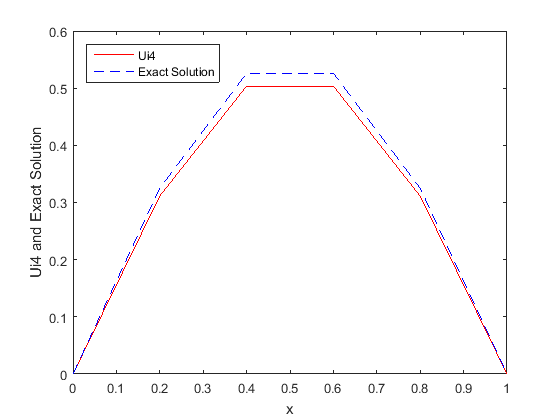
\includegraphics[width=1.1\linewidth]{graph_f}
\end{center}
\textbf{Discussion of Results}\\
From the table and graph above, the approximate solution is calculated using Bender Schmidt method with step size 0.2. It is seen that the numerical solution converges to the exact solution, although the smaller the step size, the more the numerical solution approaches the exact solution on the graph.\\

\noindent Finally, it can be seen from the results above that the Laplace Transform and the New Modified Variational Iteration Method among other analytic methods, is an effective method for solving Second Order Partial Differential Equation with boundary conditions. 



\chapter{SUMMARY AND CONCLUSION}
\section{SUMMARY}
\qquad The main aim of this project work is to use Laplace transform in combination with the new modified variational iteration method to solve linear and nonlinear partial differential equations. In the first chapter, we discussed the historical background of differential equations, stating its types, order, and degree. Also, we discussed partial differential equations, its definition, its classification, and examples. 
\par Chapter two consists of literature review in which history of partial differential equation and Laplace transform were explained.
\par Chapter three consists of the explanation on Laplace transform in which we discussed its method (how to use it), properties, the inverse laplace transform, and the laplace table. 
\par Chapter four also consists of the main work whereby we firstly use Laplace transform to solve second order linear partial differential equation, and later combined the Laplace transform method with the new modified variational iteration method to solve nonlinear partial differential equations.
\section{CONCLUSION}
\qquad In this project work, we applied a new method for solving nonlinear partial differential equations. The new method is the combination of the new modified variational iteration method and the Laplace transform method which is successfully implemented by using the initial conditions only. The method is also efficient(without wasting time) in solving linear partial differential equation.\\

The method is simple, easy to use, and gives exact solution in solving non-linear partial differential equations when enough iteration is considered. This variational iteration method will become much more interesting to solve non-linear partial differential equations in science and engineering.\\ 


\newpage
\chapter*{REFERENCES}
\addcontentsline{toc}{chapter}{REFERENCES}
\begin{description}
  \item Abassy, T.A. (2012). Modified variational iteration method (non-homogenous initial value problem). \textit{Mathematical and Computer Modelling} \textit{55}(3-4), 1222-1232.
  
  \item Alfred, K. (1994). \textit{Science and and Sanity: an Introduction to non-Aristotelian Systems and General Semantics.} (Section: Differential Equations, pg. 595). Institute of General Semantics.
  
  \item Archibald, T., Fraser, C., Grattan-Guinness, I. (2005). The History of Differential Equations, 1670-1950. \textit{Oberwolfach Reports}, \textit{1}(4), 2729-2794. 
	 \item Blurnan, G., \& Kumei, S. (1989). Symmetries and Differential Equations. 
	 
	 \item Denis, B. (2020). An Overview of Numerical and Analytical Methods for solving Ordinary Differential Equations. \textit{arXiv} preprint arXiv: 2012.07558.
	 
	 \item He, J.H. (1999). Variational Iteration Method - a kind of non-linear analytical technique: some examples. \textit{International journal of non-linear mechanics}, \textit{34}(4), 699-708.
		
		\item Poincare, H. (1890). On the partial differential equations of mathematical physics. \textit{American journal of Mathematics}, 211-294.
		
		\item Sikka, H. (2018). Differential equations and its area of applications.
		
		\item Solin, P. (2005). \textit{Partial differential equations and the finite element method} (Vol. 73). John Wiley \& Sons.
		
		\item Wazwaz, A.M. (2009). The Variational iteration method for analytic treatment for linear and non-linear ODEs. \textit{Applied Mathematics and Computation}, \textit{212}(1), 120-134. 
		
		\item Williams, J. (1973). \textit{Laplace transforms}. Allen \& Unwin.  
\end{document}
